\chapter{UrbanSim Models and Data Structures}

\section{Geographic Units of Analysis in UrbanSim Models}
UrbanSim has evolved over several years, and so have the data
structures used in it.  Until 2005, most applications used a geographic framework based on a grid overlaid on the study area.  Most UrbanSim applications to date have used this approach to structuring the data.  Various limitations of the gridcell approach led to the more recent adoption of a parcel-based data and spatial structure.  This section explains the fundamental differences in these data structures, and assesses their relative merits.  Both are still used and supported approaches, though the advantages of the parcel approach are fairly significant.  We begin with an overview of the three different data structures that UrbanSim now supports: gridcells, parcels, and zones.

%In this chapter, the Puget Sound model application is used extensively as the basis for the description, in order to make the discussion more tangible\footnote{This does not restrict the generalizability of the results, since the model has been widely adapted to multiple metropolitan areas in North America, Europe and Asia.}.  The study area for the Puget Sound model, now being brought into operational use by the Puget Sound Regional Council (PSRC), is the Central Puget Sound, consisting of King, Kitsap, Pierce and Snohomish Counties in Washington, as shown in Figure \ref{fig:puget-sound}.

%\begin{figure}
%\begin{center} 
%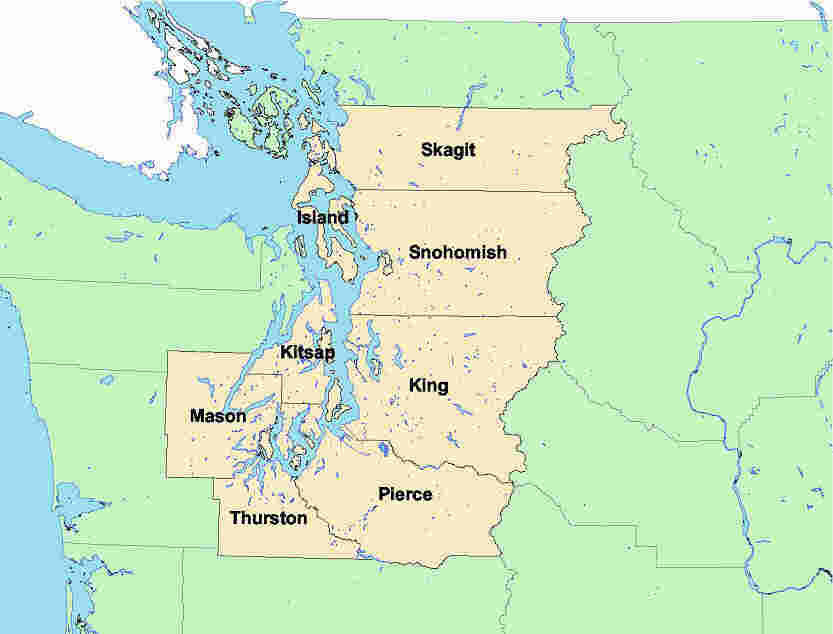
\includegraphics[scale=0.4]{graphics/psrc-p1.jpg}
%\end{center}
%\caption{Puget Sound Region} 
%\label{fig:puget-sound}
%\end{figure}


The gridcell-based approach to developing the data for UrbanSim, as the name suggests, begins with the decision of a resolution to use for a grid to overlay the study area.  There is no definitively correct grid cell resolution, and a pragmatic choice of 150 meters by 150 meters was chosen in early UrbanSim
applications, mainly as a compromise between the high level of resolution desired, and the increased computational demands made by higher resolution data.

Figure \ref{fig:gridcells} depicts a portion of the study area in the Puget Sound, and shows the 150 meter grid initially used for the PSRC model application
superimposed on other planning geographies for relative comparison.  It is obvious that grid cells bisect parcels, or to put it another way, that it is not possible to aggregate parcel information neatly into gridcells.  This was an unfortunate but obvious outcome of imposing a completely regular shape (a grid) on a polygonal layer of parcels that vary in size in shape.  The main advantage of using a grid is that is makes it possible
to use raster processing efficiently, as is done in image processing or raster GIS spatial analysis.  It is possible to compute quite efficiently, for example, how much population or employment is within a fixed radius of each cell.  This computational efficiency was the main initial motivation for using the gridcell approach to structuring the input data for UrbanSim.

\begin{figure}[htp]
\begin{center}
%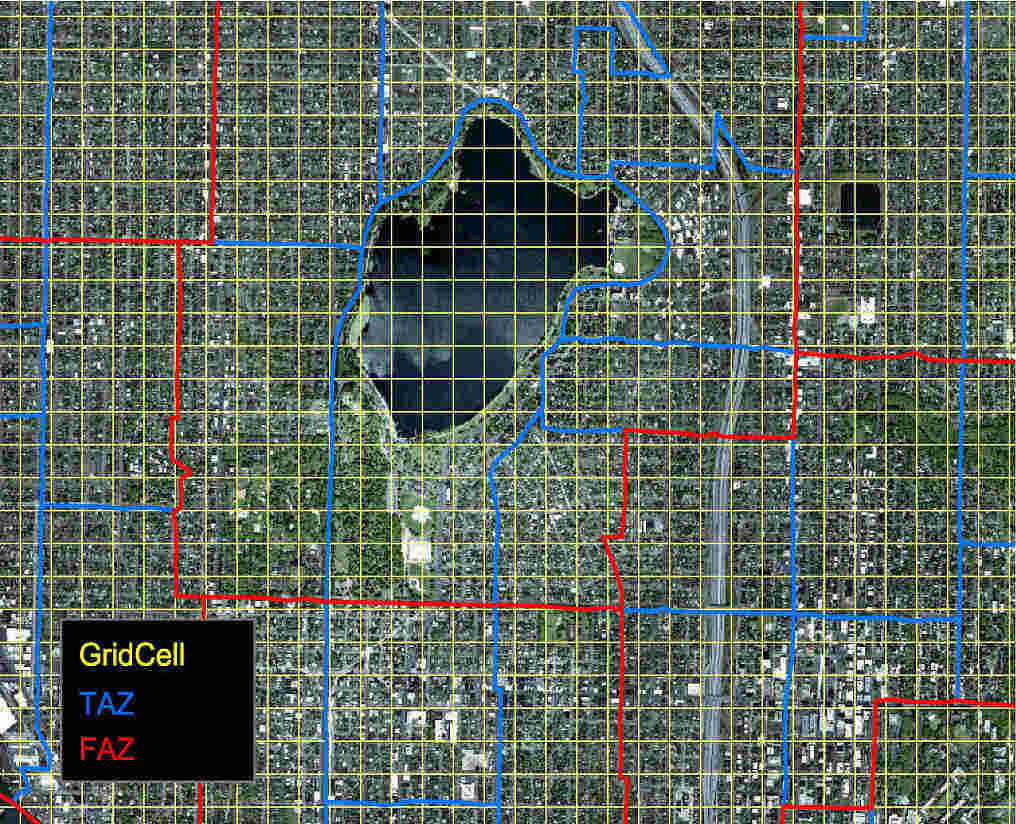
\includegraphics[scale=0.5]{graphics/grid-greenlake.jpg}
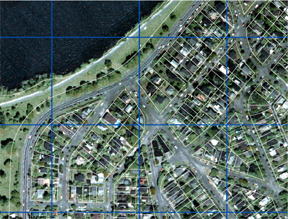
\includegraphics[scale=1.25]{graphics/gridmap-small.png}
\end{center}
\caption{Gridcells in Greenlake Area of Seattle}
\label{fig:gridcells}
\end{figure}

Each gridcell contains approximately 5 1/2 acres, at a resolution of 150 meters.  In order to prepare the data for UrbanSim, parcel maps were overlaid in the GIS on a vector representation of gridcells, and the contents of the parcel (housing, etc)  allocated to the gridcells in proportion to the amount of its land area falling within each gridcell.  The fragments of the real estate components created in this way were then aggregated into a composite at the cell level.  UrbanSim then operates on the gridcell-level data.  In order to better reflect the contents of the grid cells, which are clearly not homogeneous in their composition, building objects were created to allow at least different types of real estate in a cell to be represented by different types of buildings.  Households and jobs were then associated with buildings, and buildings with gridcells, as shown in Figure \ref{fig:flexible-geographies}.

%\begin{figure}[htp]
%\center \resizebox{0.3
%\textwidth}{!}{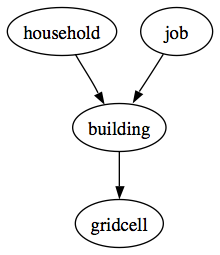
\includegraphics{graphics/grid-data-model.png}}
%\caption{Core of Gridcell-based UrbanSim Data Model} \label{fig:grid-data-model}
%\end{figure}

The main disadvantage of the gridcell data structure has already been mentioned: it requires unnaturally splitting the underlying parcel information and
recombining it in ways that create artificial representations of the data.  This problem also makes it difficult to apply information on development regulations
from general plans, since those are also based on polygons, and in fact, apply to parcels.

\begin{figure}
\centering
\subfigure[gridcell] % caption for subfigure a
{
    \label{fig:a}
    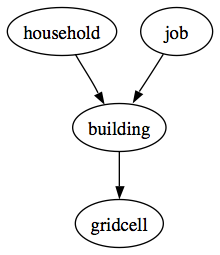
\includegraphics[width=4cm]{graphics/grid-data-model.png}
}
\hspace{1cm}
\subfigure[parcel] % caption for subfigure b
{
    \label{fig:b}
    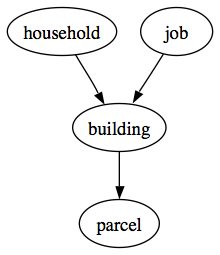
\includegraphics[width=4cm]{graphics/data-model-parcel.png}
}
\hspace{1cm}
\subfigure[zone] % caption for subfigure b
{
    \label{fig:c}
    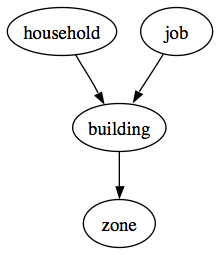
\includegraphics[width=4cm]{graphics/data-model-zone.png}
}
\caption{Flexible Geographic Units for UrbanSim}
\label{fig:flexible-geographies} % caption for the whole figure
\end{figure}




To address some of the limitations of the gridcell-based data structure, recent development of UrbanSim has adopted a data structure based on parcels.
The parcel-based UrbanSim application uses a data model that reflects parcels, buildings, households and jobs as the
primary objects and units of analysis.  Households and jobs
choose locations by selecting a specific building, which is associated with a specific parcel.
Real estate development is based on development projects occurring on specific parcels.  In the most recent extensions of the Puget Sound model,
persons have been added to the data model, and workers are associated with specific jobs.  These data relationships
are shown in Figure \ref{fig:flexible-geographies}, and make clear that only the link of buildings to a geographic unit is changed.

%\begin{figure*}[ht]
%\center \resizebox{0.3
%\textwidth}{!}{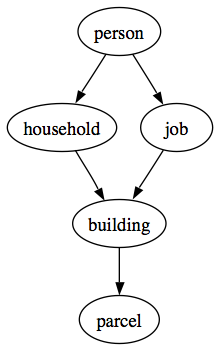
\includegraphics{graphics/data-model-2.png}}
%\caption{Core of Parcel-based UrbanSim Data Model} \label{fig:data-model-2}
%\end{figure*}


Given the available flexibility in configuring models in OPUS, an alternative data structure can be readily substituted for parcel or gridcell based data.  For example, locations could be defined by zones used in the travel model, to make them consistent with current-generation zone-based travel models.  This approach can also be used to create a rather simple model system using less geographic detail.  For example, an application in Paris used Communes, or administrative areas roughly equivalent to traffic analysis zones in number (approximately 1300).

By using the same data structure for households, jobs and buildings, the only change needed for a zone-based model system is to assign locations to buildings at a coarser level of detail, such as the zone.  This retains all of the accounting systems in the UrbanSim model: households and jobs are still located in buildings, and buildings can be added to zones.  But this approach would give up considerable detail for analyzing development locations and capacity constraints due to zoning or land use plans. For testing purposes, a zone-based model system has been implemented in UrbanSim and is being prepared for access via the GUI.

%Data from the four counties that comprise the Central Puget Sound - King, Kitsap, Pierce, and Snohomish, shown in Figure \ref{fig:puget-sound} - were assembled to create a year 2000 database\footnote{2001 parcel data were obtained from the assessor files for each county, since there are considerable lags in updating these data
%and also due to some significant gaps in the 2000 data from Snohomish County}.  Over 1.2 million parcels are represented in the UrbanSim database
%for the Puget Sound, containing over 1 million buildings, almost 1.4 million residential units, and over 1 billion square feet of non-residential space.  Individual building records were separately obtained from two of the counties (King and Snohomish), and were created from
%the parcel data attributes for the other two counties.  Attributes of the core datasets are shown in Table \ref{tab:parcel-attributes}. Attributes of the core datasets are shown in Table \ref{tab:parcel-attributes}.

%\begin{figure*}
%\center \resizebox{0.9
%\textwidth}{!}{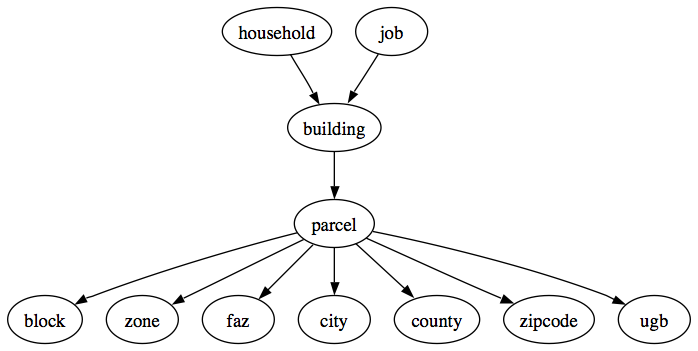
\includegraphics{graphics/geographic-relationships.png}}
%\caption{Spatial Relationships Among Core UrbanSim Entities} \label{fig:geographic-relationships}
%\end{figure*}



\section{UrbanSim Model Components}

The overall architecture of the UrbanSim model system is depicted in Figure \ref{fig:urbansim-overview}.  


\begin{figure}[htp]
\center
 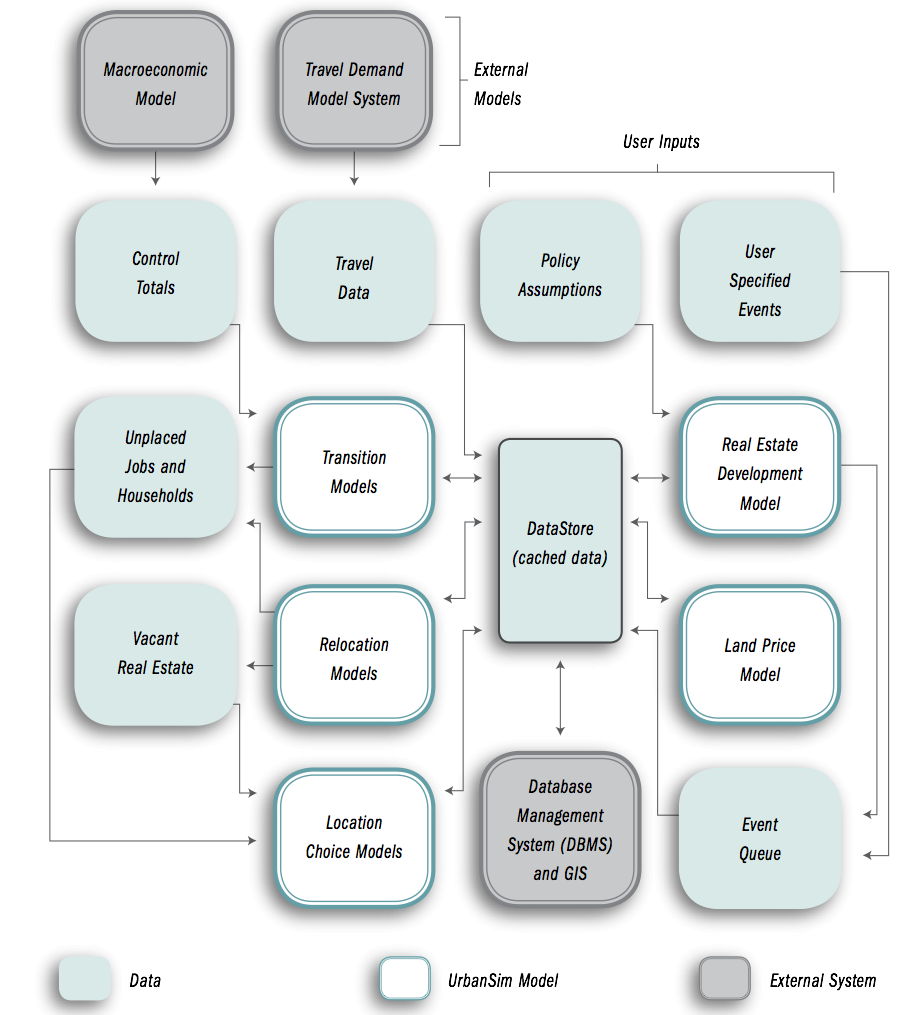
\includegraphics[width=6.5in]
 {graphics/urbansim-overview.png}
\caption{Overview of UrbanSim Model System}
\label{fig:urbansim-overview}
\end{figure}

The models used in the parcel version of UrbanSim differ in some obvious respects from the earlier gridcell versions, and these are summarized in Table \ref{tab:components-parcel}.  In addition to the substitution of parcels for gridcells as the unit of analysis, the real estate development model was completely restructured to take advantage of the availability of parcel geography in representing actual development projects - which do vary in size and shape in the real world, in ways that were difficult to reconcile with gridcell geography.  The parcel based model specifications also have recently added models to predict the choice of workers to be home-based (normally work from home), and a workplace choice model for workers who are not home-based.  This allows for the first time the more appropriate handling of the prediction of commuting behavior as a long-term outcome of where a household chooses to live, and where the workers in the household have jobs, and allows the removal of the home-based-work trip distribution model from the set of behaviors predicted by the travel model on a daily basis.

\begin{table}[htp]
\caption{Specification of UrbanSim Model Components Using Parcel Data Structure}
\label{tab:components-parcel}
%\begin{tabular*}{6in}{@{\extracolsep{\fill}}  p{5cm} | p{.2cm} | p{2cm} | p{2.5cm} | p{2cm} | }
\begin{tabular}{p{4.5cm} p{3.4cm}p{3.4cm}p{3.3cm}}
\toprule[1.5pt]
Model & Agent & Dependent Variable & Functional Form \\
\midrule
Household Location Choice & Household (New or Moving) & Residential Building With Vacant Unit & Multinomial Logit \\
\midrule
Employment Location Choice & Job (New or Moving) & Non-residential Building With Vacant Space & Multinomial Logit \\
\midrule
Home-based Job Choice & Worker (Without Job) & Binary Choice (Work at Home) & Binary Logit \\
\midrule
Workplace Choice & Non Home Based Worker (Without Job) & Vacant Job & Multinomial Logit \\
\midrule
Real Estate Development  & Development Proposal & Parcel (With Vacant Land) & Multinomial Logit Sampler \\
\midrule
Real Estate Price & Parcel & Price Per Square Foot & Multiple Regression \\
\bottomrule[1.5pt]
\end{tabular}
\end{table}


In the remainder of this chapter, the components of the current version of UrbanSim
are described in some detail in terms of their
structure and algorithms.  Since many (but not all) of these models are based on a discrete choice framework,
a brief explanation of the common basis for these models is presented first.  Where model specifications
vary by geographic basis (e.g. gridcell or parcel), deviations are described.  First, the common underpinnings
of many of the models, discrete choice models, is presented as an overview.

\subsection{Discrete Choice Models}
\label{sec:discrete-choice}

A pathbreaking approach to modeling individual actions using discrete
choice models emerged in the 1970's, with the pioneering work of
McFadden on Random Utility Maximization theory
\cite{mcfadden-1974,mcfadden-1981}. This approach derives a model of
the probability of choosing among a set of available alternatives
based on the characteristics of the chooser and the attributes of
the alternative, and proportional to the relative utility that the
alternatives generate for the chooser. Maximum likelihood and
simulated maximum likelihood methods have been developed to estimate
the parameters of these choice models from data on revealed or
stated preferences, using a wide range of structural specifications
(see \cite{train-book-2003}). Early application of these models were
principally in the transportation field, but also included work on
residential location choices
\cite{quigley-eer-1976,lerman-trr-1977,mcfadden-1978}, and
on residential mobility \cite{clark-vanlierop-1986}.

Let us begin with an example of a simple model of households choosing among
alternative locations in the housing market, which we index by
$i$. For each agent, we assume that each alternative $i$ has
associated with it a utility $U_i$ that can be separated into a
systematic part and a random part:
\begin{equation}
    U_i = V_i + \epsilon_i,
    \label{eq:utility}
\end{equation}
%$V_i = \vk{\beta}\cdot\vk{x}_i$
where $V_i = \beta\cdot {x}_i$ is a linear-in-parameters
function, $\beta$ is a vector of $k$ estimable coefficients,
$x_i$ is a vector of observed, exogenous, independent
alternative-specific variables that may be interacted with the
characteristics of the agent making the choice, and $\epsilon_i$
is an unobserved random term. Assuming the unobserved term in
(\ref{eq:utility}) to be distributed with a Gumbel distribution
leads to the  widely used multinomial logit model
\cite{mcfadden-1974,mcfadden-1981}:
\begin{equation}
    P_i = \frac{\mathrm{e}^{V_i}}{\sum_j \mathrm{e}^{V_j}},
    \label{eq:mnl}
\end{equation}
where $j$ is an index over all possible alternatives. The
estimable coefficients of (\ref{eq:mnl}), $\beta$, are
estimated with the method of maximum likelihood (see for example
\cite{greene-2002}).

The denominator of the equation for the choice model has a particular
significance as an evaluation measure.  The log of this denominator
is called the \emph{logsum}, or composite utility, and it summarizes
the utility across all the alternatives.  In the context of a choice of
mode between origins and destinations, for example, it would summarize
the utility (disutility) of travel, considering all the modes connecting the
origins and destinations.  It has theoretical appeal as an evaluation
measure for this reason.  In fact, the logsum from the mode choice
model can be used as a measure of accessibility.

\begin{figure}[htp]
\center
 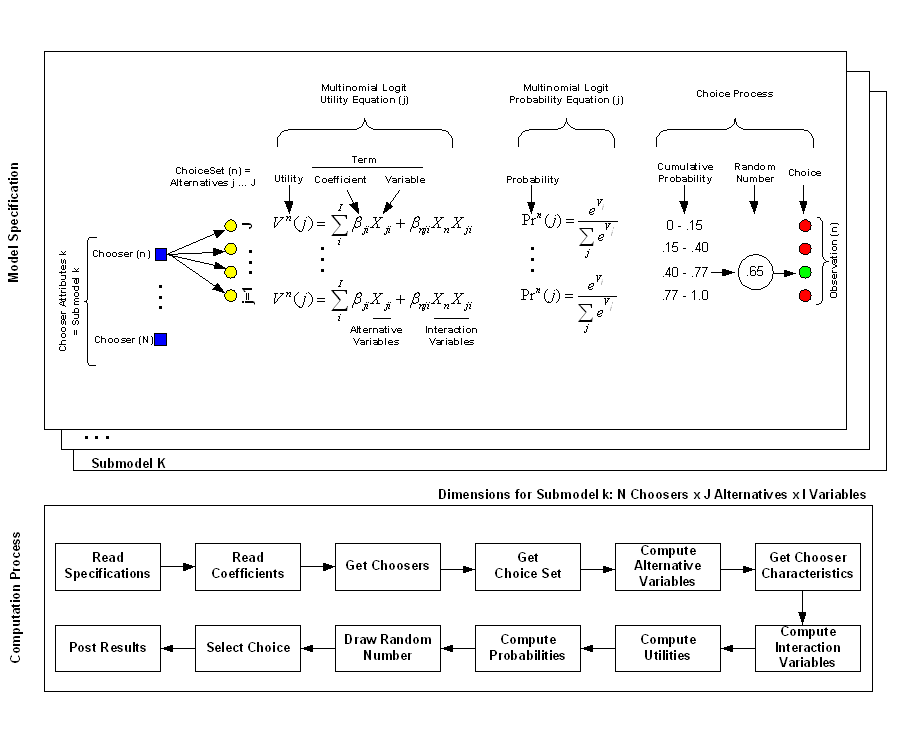
\includegraphics[width=6.5in]
 {graphics/ChoiceProcess.png}
\caption{Computation Process in UrbanSim Choice Models}
\label{fig:choiceprocess}
\end{figure}

Choice models are implemented in UrbanSim in a modular way, to allow flexible specification of models
to reflect a wide variety of choice situations.  Figure \ref{fig:choiceprocess} shows the process both in the form
of the equations to be computed, and from the perspective of the tasks implemented as methods in software.

For each model component within the UrbanSim model system, the
choice process proceeds as shown in Figure
\ref{fig:choiceprocess}. The first steps of the model read the
relevant model specifications and data.  Then a choice set is
constructed for each chooser.  Currently this is done using random
sampling of alternatives, which has been shown to generate consistent, though not
efficient, estimates of model parameters \cite{ben-akiva-lerman-1987}.

The choice step in this algorithm warrants further explanation.  Choice models predict choice probabilities, not choices.
In order to predict choices given the predicted probabilities, we require an algorithm to select a specific choice outcome.
A tempting approach would be to select the alternative with the maximum probability, but unfortunatelty this strategy
would have the effect of selecting only the dominant outcome, and less frequent alternatives would be completely
eliminated.  In a mode choice model, for illustration, the transit mode would disappear, since the probability of choosing
an auto mode is almost always higher than that of choosing transit.  Clearly this is not a desirable or realistic outcome.
In order to address this problem, the choice algorithm used for choice models uses a sampling approach.  As illustrated in Figure
\ref{fig:choiceprocess}, a choice outcome can be selected by sampling a random number from the uniform distribution in the range
0 to 1, and comparing this random draw to the cumulative probabilities of the alternatives.  Whichever alternative the sampled
random number falls within is the alternative that is selected as the `chosen' one.  This algorithm has the property that it
preserves in the distribution of choice outcomes a close approximation of the original probability distribution, especially
as the sample size of choosers becomes larger.

One other choice context is worth noting.  In some situations, the availability of alternatives may be constrained.  If the limit on availability
is entirely predictable, such as a budget constraint eliminating expensive options, or a zero-car household being unable to use the drive-alone
mode, this is straightforward to handle, by eliminating the alternatives from the choice set for those choosers.  In other situations, however, the
solution is not so straightforward.  In the case where alternatives may be unavailable because many other agents wish to choose them, the problem
is that the alternative may be unavailable due to the endogenous congestion of alternatives.  The effect of this is potentially significant, since it
may cause parameters estimated in a choice model to confuse, or confound, the effects of preferences with the effects of constraints.  Fortunately,
an estimation method has been developed to account for this problem \cite{depalma-jue-2007}.

\subsection{Economic Transition Model}
Employment is classified by the user into employment sectors based
on aggregations of Standard Industrial Classification (SIC) codes, or more
recently, North American Industry Classification (NAICS) codes.
Typically 10 to 20 sectors are defined based on the local economic
structure. Aggregate forecasts of economic activity and sectoral
employment are exogenous to UrbanSim, and are used as inputs to
the model. These forecasts may be obtained from state economic
forecasts or from commercial or in-house sources.

The base year UrbanSim employment data for the
Puget Sound application are derived from data from the State of Washington
Employment Securities Division, generally referred to
as ES202 data, containing unemployment insurance administrative
records with information on the location and size of business
establishments.  InfoUSA is a commonly used private source for
similar data, compiled from credit reports and other sources.

The Economic Transition Model integrates exogenous forecasts
of aggregate employment by sector with the UrbanSim database by
computing the sectoral growth or decline from the preceding year,
and either removing jobs from the database in sectors that are
declining, or queuing jobs to be placed in the employment location
choice model for sectors that experience growth.  If the user
supplies only total employment control totals, rather than totals
by sector, the sectoral distribution is assumed consistent with
the current sectoral distribution. In cases of employment loss,
the probability that a job will be removed is assumed proportional
to the spatial distribution of jobs in the sector.  The jobs that
are removed vacate the space they were occupying, and this space
becomes available to the pool of vacant space for other jobs to
occupy in the location component of the model.  This procedure
keeps the accounting of land, structures, and occupants up to
date.

New jobs are not immediately assigned a location.  Instead, new
jobs are added to the database and assigned a null location, to be
resolved by the Employment Location Choice Model.


\subsection{Demographic Transition Model}

The Demographic Transition Model accounts for changes in the
distribution of households by type over time, using an algorithm
analogous to that used in the Economic Transition Model.  In
reality, these changes result from a complex set of social and
demographic changes that include aging, household formation,
divorce and household dissolution, mortality, birth of children,
migration into and from the region, changes in household size, and
changes in income, among others.  The data (and theory) required
to represent all of these components and their interactions
adequately are complex, and this set of behaviors remain to be
implemented in UrbanSim. Instead, the Demographic
Transition Model, like the Economic Transition Model described
above, uses external control totals of population and households
by type (the latter only if available) to provide a mechanism for
the user to approximate the net results of these changes. Analysis
by the user of local demographic trends may inform the
construction of control totals with distributions of household
size, age of head, and income.  If only total population is
provided in the control totals, the model assumes that the
distribution of households by type remains static.

As in the economic transition case, household births are added to
a list of movers that will be located by the Household Location
Choice Model.  Household deaths, on the other hand, are accounted
for by this model by removing those households from the housing
stock, and by properly accounting for the vacancies created by
their departure.  The demographic transition model is analogous in
form to the employment transition model described above.


\subsection{Employment Relocation Choice Model}

Employment relocation and location choices are made by firms.
However, in the current version of UrbanSim, we use individual
jobs as the units of analysis.  This is equivalent to assuming
that businesses are making individual choices about the location
of each job, and are not constrained to moving an entire
establishment.

The Employment Relocation Choice Model predicts the probability that jobs
of each type will move from their current location or stay during
a particular year. This is a transitional change that could
reflect job turnover by employees, layoffs, business relocations
or closures. Similar to the economic transition model when
handling job losses in declining sectors, the model assumes that
the hazard of moving is proportional to the spatial distribution
of jobs in the sector.  All placement of jobs is managed through
the employment location model.

As in the case of job losses predicted in the economic transition
component, the application of this model requires subtracting jobs
by sector from the buildings they currently occupy, and the
updating of the accounting to make this space available as vacant
space. These counts will be added to the unallocated new jobs by
sector calculated in the economic transition model. The
combination of new and moving jobs serve as a pool to be located
in the employment location choice model. Vacancy of nonresidential
space will be updated, making space available for allocation in
the employment location choice model.

Since it is possible that the relative attractiveness of
commercial space in other locations when compared with an
establishment's current location may influence its decision to
move, an alternative structure for the mobility model could use
the marginal choice in a nested logit model with a conditional
choice of location. In this way, the model would use information
about the relative utility of alternative locations compared to
the utility of the current location in predicting whether jobs
will move.  While this might be more theoretically appealing than
the specification given, it is generally not supported by the data
available for calibration. Instead, the mobility decision is
treated as an independent choice, and the probabilities estimated
by annual mobility rates directly observed over a recent period
for each sector.


\subsection{Household Relocation Choice Model}

The Household Relocation Choice Model is similar in form to the Employment
Relocation Choice Model described above.  The same algorithm is used, but
with rates or coefficients applicable to each household type.  For
households, mobility probabilities are estimated from the Census
Current Population Survey, which provides a national database on
which annual mobility rates are computed by type of household.
This will reflect differential mobility rates for renters and
owners, and households at different life stages.

Application of the Household Relocation Choice Model requires subtracting
mover households by type from the housing stock by building, and
adding them to the pool of new households by type estimated in the
Demographic Transition Model. In the database, this is
accomplished by setting the location field for the moving
households to a null value.  The combination of new and moving
households serves as a population of households to be located by
the Household Location Choice Model. Housing vacancy is updated as
movers are subtracted, making the housing available for occupation
in the household location and housing type choice model.


\subsection{Employment Location Choice Model}

In this model, we predict the probability that a job that is
either new (from the Economic Transition Model), or has moved
within the region (from the Employment Mobility Model), will be
located at a particular site.  Buildings are used as the basic
geographic unit of analysis in the current model implementation.
Each job has an attribute of space it needs, and this provides
a simple accounting framework for space utilization within
buildings. The
number of locations available for a job to locate within a building
will depend mainly on the total square footage of
nonresidential floorspace in the building, and on the density of the
use of space (square feet per employee).

Given the possibility
that some jobs will be located in residential units, however,
housing as well as nonresidential floorspace must be considered in
job location.  We have allowed the user to specify the control totals
for employment by sector in two categories: home-based and
non-home-based.  The model is specified as a multinomial logit model,
with separate equations estimated for each employment sector.


For both the employment location and household location models, we
take the stock of available space as fixed in the short run of the
intra-year period of the simulation, and assume that locators are
price takers.  That is, a single locating job or household does
not have enough market power to influence the transaction price,
and must accept the current market price as given.

The variables included in the employment location choice model are
drawn from the literature in urban economics.  We expect that
accessibility to population, particularly high-income population,
increases bids for retail and service businesses.  We also expect
that two forms of agglomeration economies influence location
choices: localization economies and inter-industry linkages.

Localization economies represent positive externalities associated
with locations that have other firms in the same industry nearby.
The basis for the attraction may be some combination of a shared
skilled labor pool, comparison shopping in the case of retail,
co-location at a site with highly desirable characteristics, or
other factors that cause the costs of production to decline as
greater concentration of businesses in the industry occurs.  The
classic example of localization economies is Silicon Valley.
Inter-industry linkages refer to agglomeration economies
associated with location at a site that has greater access to
businesses in strategically related, but different, industries.
Examples include manufacturers locating near concentrations of
suppliers in different industries, or distribution companies
locating where they can readily service retail outlets.

One complication in measuring localization economies and
inter-industry linkages is determining the relevant distance for
agglomeration economies to influence location choices.  At one
level, agglomeration economies are likely to affect business
location choices between states, or between metropolitan areas
within a state.  Within a single metropolitan area, we are
concerned more with agglomeration economies at a scale relevant to
the formation of employment centers.  The influence of proximity
to related employment may be measured using two scales: a regional
scale effect using zone-to-zone accessibilities from the travel
model, or highly localized accessibilities using queries of the
area immediately around the given parcel.  Most of the spatial
queries used in the model are of the latter type, because the
regional accessibility variables tend to be very highly
correlated, and because agglomerations are expected to be very
localized.

Age of buildings is included in the model to estimate the
influence of age depreciation of commercial buildings, with the
expectation that businesses prefer newer buildings and discount
their bids for older ones.  This reflects the deterioration of
older buildings, changing architecture, and preferences, as is the
case in residential housing.  There is the possibility that
significant renovation will make the actual year built less
relevant, and we would expect that this would dampen the
coefficient for age depreciation.  We do not at this point attempt
to model maintenance and renovation investments and the quality of
buildings.

Density, the inverse of lot size, is included in the location
choice model.  We expect businesses, like households, to reveal
different preferences for land based on their production functions
and the role of amenities such as green space and parking area. As
manufacturing production continues to shift to more horizontal,
land-intensive technology, we expect the discounting for density
to be relatively high.  Retail, with its concentration in shopping
strips and malls, still requires substantial surface land for
parking, and is likely to discount bids less for density.  We
expect service firms to discount for density the least, since in
the traditional urban economics models of bid-rent, service firms
generally outbid other firms for sites with higher accessibility,
land cost, and density.

We might expect that certain sectors, particularly retail, show
some preference for locations near a major highway, and are
willing to bid higher for those locations.  Distance to a highway
is measured in meters, using grid spatial queries.  We also test
for the residual influence of the classic monocentric model,
measured by travel time to the CBD, after controlling for
population access and agglomeration economies.  We expect that,
for most regions, the CBD accessibility influence will be
insignificant or the reverse of that in the traditional
monocentric model, after accounting for these other effects.

Estimation of the parameters of the model is based on a geocoded establishment file
(matched to the parcel file to link employment by type to land use
by type).  A sample of geocoded jobs in each sector is used to
estimate the coefficients of the location choice model.  As with
the Household Location Choice Model, the application of the model
produces demand by each employment type for building locations.

The independent variables used in the employment location choice
model can be grouped into the categories of real estate
characteristics, regional accessibility, and urban-design scale
effects as shown below:

\begin{itemize}

\item Real Estate Characteristics \\ \emph{Prices} \\
\emph{Development type (land use mix, density)}

\item Regional accessibility \\
\emph{Access to population} \\ \emph{Travel time to CBD, airport}

\item Urban design-scale \\ \emph{Proximity to highway, arterials}

\item Local agglomeration economies within and between sectors: center
formation

\end{itemize}



\subsection{Household Location Choice Model}

In this model, as in the employment location model, we predict the
probability that a household that is either new (from the
transition component), or has decided to move within the region
(from the mobility component), will choose a particular location
defined by a residential building.  As before, the form of the model is
specified as multinomial logit, with random sampling of
alternatives from the universe of available (vacant) housing
units, including those units vacated by movers in the current
year.

The model architecture allows location choice models to be
estimated for households stratified by income level, the presence
or absence of children, and other life cycle characteristics.
Alternatively, these effects can be included in a single model
estimation through interactions of the household characteristics
with the characteristics of the alternative locations.  The
current implementation is based on the latter but is general
enough to accommodate stratified estimation, for example by
household income. The variables used in the model are drawn from
the literature in urban economics, urban geography, and urban
sociology.  An initial feature of the model specification is the
incorporation of the classical urban economic trade-off between
transportation and land cost. This has been generalized to account
not only for travel time to the classical monocentric center, the
CBD, but also to more generalized access to employment
opportunities and to shopping. These accessibilities to work and
shopping are measured by weighting the opportunities at each
destination zone with a composite utility of travel across all
modes to the destination, based on the logsum from the mode choice
travel model.

These measures of accessibility should negate the traditional pull
of the CBD, and, for some population segments, potentially reverse
it.  In addition to these accessibility variables, we include in
the model a net building density, to measure the
input-substitution effect of land and capital.  To the extent that
land near high accessibility locations is bid up in price, we
should expect that builders will substitute capital for land and
build at higher densities.  Consumers for whom land is a more
important amenity will choose larger lot housing with less
accessibility, and the converse should hold for households that
value accessibility more than land, such as higher income
childless households.

The age of housing is considered for two reasons.  First, we
should expect that housing depreciates with age, since the
expected life of a building is finite, and a consistent stream of
maintenance investments are required to slow the deterioration of
the structure once it is built.  Second, due to changing
architectural styles, amenities, and tastes, we should expect that
the wealthiest households prefer newer housing, all else being
equal.  The exception to this pattern is likely to be older,
architecturally interesting, high quality housing in historically
wealthy neighborhoods.  The preference for these alternatives are
accommodated through a combination of nonlinear or dummy variable
treatment for this type of housing and neighborhood.

A related hypothesis from urban economics is that, since housing
is considered a normal good, it has a positive income elasticity
of demand.  This implies that as incomes rise, households will
spend a portion of the gains in income to purchase housing that is
more expensive, and that provides more amenities (structural and
neighborhood) than their prior dwelling.  A similar hypothesis is
articulated in urban sociology in which upward social mobility is
associated with spatial proximity to higher status households.
Both of these hypotheses predict that households of any given
income level prefer, all else being equal, to locate in
neighborhoods that have higher average incomes.  (UrbanSim does
not attempt to operationalize the concepts of social status or
social assimilation, but does consider income in the location
choice.)

The age hypothesis and the two income-related hypotheses are
consistent with the housing filtering model, which explains the
dynamic of new housing construction for wealthy households that
sets in motion a chain of vacancies.   The vacancy chain causes
households to move into higher status neighborhoods than the ones
they leave, and housing units to be successively occupied by lower
and lower status occupants.  At the end of the vacancy chain, in
the least desirable housing stock and the least desirable
neighborhoods, there can be insufficient demand to sustain the
housing stock and vacancies go unsatisfied, leading ultimately to
housing abandonment.  We include in the model an age depreciation
variable, along with a neighborhood income composition set of
variables, to collectively test the housing filtering and related
hypotheses.

Housing type is included in the model as a set of dummy variables
for alternative housing types.  These
are discussed further in Section
\ref{real-estate-development-model} describing the real estate
development model.

One of the features that households prefer is a compatible land
use mix within the neighborhood.  It is likely that residential
land use, as a proxy for land uses that are compatible with
residential use, positively influences housing bids.   On the
other hand, industrial land use, as a proxy for less desirable
land use characteristics, would lower bids.

The model parameters are estimated using a random sample of alternative
locations, which has been shown to provide consistent estimates of
the coefficients.  In application for forecasting, each locating
household is modeled individually, and a sample of alternative
cell locations is generated in proportion to the available
(vacant) housing. Monte carlo simulation is used to select the
specific alternative to be assigned to the household, and vacant
and occupied housing units are updated in the cell.

The market allocation mechanism used to assign households and jobs
to available space, then, is not done through a general
equilibrium solution in which we assume consumers and suppliers
optimize across all alternatives based on perfect information, and
zero transaction costs, with prices on all buildings at each
location adjusting to the general equilibrium solution that
perfectly matches consumers and suppliers to clear the market.
Rather, the solution is based on an expectation of incomplete
information and nontrivial transactions and search costs, so that
movers obtain the highest satisfactory location that is available,
and prices respond at the end of the year to the balance of demand
and supply at each location.

The independent variables can be organized into the three
categories of housing characteristics, regional accessibility, and
urban-design scale effects as shown below.

\begin{itemize}

\item{Housing Characteristics} \\
\emph{Prices (interacted with income) \\
Development types (density, land use mix) Housing age}

\item{Regional accessibility} \\
\emph{Job accessibility by auto-ownership group \\
Travel time to CBD and airport}

\item{Urban design-scale (local accessibility) \\
\emph{Neighborhood land use mix and density \\
Neighborhood Employment}}

\end{itemize}

\subsection{Real Estate Price Model}

UrbanSim uses real estate prices as the indicator of the match between
demand and supply of land at different locations and with
different land use types, and of the relative market valuations
for attributes of housing, nonresidential space, and location.
This role is important to the rationing of land and buildings to
consumers based on preferences and ability to pay, as a reflection
of the operation of actual real estate markets. Since prices enter
the location choice utility functions for jobs and households, an
adjustment in prices will alter location preferences.  All else
being equal, this will in turn cause higher price alternatives to
become more likely to be chosen by occupants who have lower price
elasticity of demand. Similarly, any adjustment in land prices
alters the preferences of developers to build new construction by
type of space, and the density of the construction.

We make the following assumptions:

\begin{enumerate}
\item Households, businesses, and developers are all
price-takers, and market adjustments are made by the market in
response to aggregate demand and supply relationships.  Each
responds, therefore, to previous period price information.

\item
Location preferences and demand-supply imbalances are capitalized
into land values.  Building value reflects building replacement
costs only, and can include variations in development costs due to
terrain, environmental constraints or development policy.

\item
There is a long-term structural vacancy rate for each type of
property, and the relationship of current vacancy rates to this
long-term vacancy rate influences price adjustments.
\end{enumerate}

Real estate prices are modeled using a hedonic regression of the log-transformed
property value per square foot
on attributes of the parcel and its environment, including land use
mix, density of development, proximity of highways and other
infrastructure, land use plan or zoning constraints, and
neighborhood effects.  The hedonic regression may be estimated
from sales transactions if there are sufficient transactions on
all property types, and if there is sufficient information on the
lot and its location.  An alternative is to use tax assessor
records on land values, which are part of the database typically
assembled to implement the model.  Although assessor records may
contain biases in their assessment, they do provide virtually
complete coverage of the land (with notable exceptions and gaps
for exempt or publicly owned property).

The hedonic regression equation encapsulates interactions between
market demand and supply, revealing an envelope of implicit
valuations for location and structural characteristics \cite{dipasquale-wheaton-1996}.
Prices are updated by UrbanSim annually, after all construction and market
activity is completed.  These end of year prices are then used as
the values of reference for market activities in the subsequent
year.

The independent variables influencing land prices can be organized
into site characteristics, regional accessibility, and urban-design
scale effects, as shown below:

\begin{itemize}

\item Site characteristics \\
\emph{Development type \\
Land use plan \\
Environmental constraints}

\item Regional accessibility \\
\emph{Access to population and employment}

\item Urban design-scale \\
\emph{Land use mix and density \\
Proximity to highway and arterials}

\end{itemize}

\subsection{Real Estate Development Model}
\label{real-estate-development-model}

\emph{WARNING: THIS SECTION STILL NEEDS TO BE UPDATED}

Constraints on development outcomes are included through a
combination of user-specified spatial overlays and decision rules
about specific types of development allowed in different
situations.  First, each parcel is assigned a series of overlays
through spatial preprocessing using GIS overlay techniques.  These
overlays include features such as the following:

\begin{itemize}
\item  Land use plan designation
\item  City
\item  County
\item  Wetland designation
\item  Floodplain/floodway
\item  Stream or riparian buffer
\item  High slope areas
\item  Urban Growth Boundary
\end{itemize}


These overlays can be used to assign user-specified constraints on
the type of development that is allowed to occur within each of
these overlay designations.  These constraints are interpreted as
'binding' constraints, and not subject to
market pressure. Currently, if users wish to examine the impact of
these constraints, they would need to 'relax' a particular
constraint within one scenario and compare the scenario results to
a more restrictive policy.

The independent variables used in the real estate development
model can be organized into categories of site characteristics,
urban design-scale effects, regional accessibility, and market
conditions, as shown below:

\begin{itemize}
\item Site characteristics \\
\emph{Existing development characteristics \\
Land use plan \\
Environmental constraints}

\item Urban design-scale \\
\emph{Proximity to highway and arterials \\
Proximity to existing development \\
Neighborhood land use mix and property values \\
Recent development in neighborhood}

\item Regional accessibility \\
\emph{Access to population and employment \\
Travel time to CBD, airport}

\item Market Conditions \\
\emph{Vacancy rates}
\end{itemize}

\subsection{The Role of Accessibility}

Accessibility is a very important influence in urban space, and it
similarly plays an important role in UrbanSim.  Almost all models
in UrbanSim consider the effects of accessibility.  But unlike
the monocentric or spatial interaction models, in which the choice
of workplace is exogenous and
residential locations are chosen principally on the basis of
commute to the city center or to a predetermined workplace, we
deal with accessibility in a more general framework. Accessibility
is considered a normal good, like other positive attributes of
housing, which consumers place a positive economic value on.  We
therefore expect that consumers value access to workplaces and
shopping opportunities, among the many other attributes they
consider in their housing preferences. However, not all households
respond to accessibility in the same way. Retired persons would be
less influenced by accessibility to job opportunities than would
working age households, for instance.

We operationalize the concept of accessibility for a given
location as the distribution of opportunities weighted by the
travel impedance, or alternatively the utility of travel to those
destinations.  A number of alternative accessibility measures have
been developed in UrbanSim. The utility of travel is measured as the composite
utility across all modes of travel for each zone pair, obtained as
the logsum of the mode choice for each origin-destination pair.

The accessibility model reads the logsum matrix from the travel
model and the land use distribution for a given year, and creates
accessibility indices for use in the household and business
location choice models. The general framework is to summarize the
accessibility from each zone to various activities for which
accessibility is considered important in household or business
location choice.

Since UrbanSim operates annually, but travel model updates are
likely to be executed for two to three of the years within the
forecasting horizon, travel utilities remain constant from one
travel model run until they are replaced by the next travel model
result. Although travel utilities remain constant, the activity
distribution in these accessibility indices is updated annually,
so that the accessibility indices change from one year to the next
to reflect the evolving spatial distribution of activities.

\subsection{User-Specified Events}

Given our current understanding, no model will be able to simulate
accurately the timing, location and nature of major events such as
a major corporate relocation into or out of a metropolitan area,
or a major development project such as a regional shopping mall.
In addition, major policy events, such as a change in the land use
plan or in an Urban Growth Boundary, are outside the range of
predictions of our simulation.  (At least in its current form,
UrbanSim is intended as a tool to aid planning and civic
deliberation, not as a tool to model the behavior of voters or
governments.  We want it to be used to say ``if you adopt the
following policy, here are the likely consequences," but not to
say ``UrbanSim predicts that in 5 years the county will adopt the
following policy.")

However, planners and decision-makers often have information about
precisely these kinds of major events, and there is a need to
integrate such information into the use of the model system.  It
is useful, for example, to explore the potential effects of a
planned corporate relocation by introducing user-specified events
to reflect the construction of the corporate building, and the
relocation into the region (and to the specific site) of a
substantial number of jobs, and examine the cumulative or
secondary effects of the relocation on further residential and
employment location and real estate development choices. Inability
to represent such events, in the presence of knowledge about
developments that may be `in the pipeline,' amounts to less than
full use of the available information about the future, and could
undermine the validity and credibility of the planning process.
For these reasons, support for three kinds of events has been
incorporated into the system: development events, employment
events, and policy events.


\section{Interface with Travel Model}

UrbanSim takes several key inputs as exogenous, meaning that these
are input assumptions that are not predicted directly by UrbanSim.  Two of these are
from external model systems: a macroeconomic model to predict
future macroeconomic conditions such as population and employment
by sector, and a travel demand model system to predict travel
conditions such as congested times and composite utilities of
travel between each interchange.  The latter is loosely coupled to
UrbanSim, with land use predictions input to the external travel
models, and travel conditions input to subsequent annual
iterations of the UrbanSim land use model system.

The travel models in widespread use in Metropolitan Planning Organizations are
almost all traditional four-step travel models.  The first model in the process
is the trip generation model, and this uses zonal population and employment
characteristics.  When UrbanSim is connected to a travel model system,
it generates a summary of the household and job data to a zone level, in order
to create the summary input data needed by the travel model.

When the travel model completes the fourth step of traffic assignment to a
transportation network, it can produce `skims' from zone to zone that summarize
key model predictions, such as:

\squishlist
\item   Travel time by mode by time of day by purpose
\item Trips by mode by time of day by purpose
\item   Composite utility of travel using all modes by purpose
\item Generalized costs (time + time equivalent of tolls) by purpose
\item Logsums, or composite utilities\footnote{See section \ref{sec:discrete-choice} for an explanation of this measure.}, from the mode choice model, by purpose and time of day
\squishend

These skims can be combined with the spatial information in UrbanSim regarding the location of households and jobs, to produce
a variety of accessibility measures, which in turn can influence UrbanSim models of residential location, workplace location, employment
location, real estate prices, and real estate development.  Figure \ref{fig:TMinterface} summarizes the interactions between UrbanSim and
the travel model system.

\begin{figure*}[ht]
\center \resizebox{0.5
\textwidth}{!}{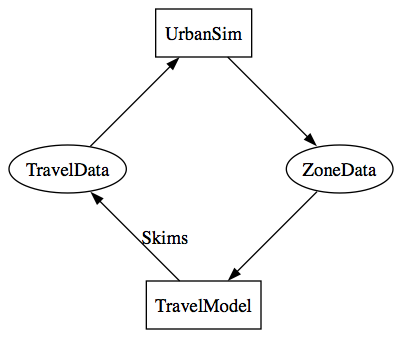
\includegraphics{graphics/travel-model-interface.png}}
\caption{UrbanSim - Travel Model Interface} \label{fig:TMinterface}
\end{figure*}

In some applications, such as the San Francisco model, the travel model system is based on a more sophisticated activity-based
framework, and UrbanSim is interfaced in a similar way. In the future, potential exists to more closely integrate UrbanSim with
Activity-based models that are moving from research into practice.


